\documentclass{report}
\usepackage{listings}
\usepackage{underscore}
\usepackage{vhistory}
\usepackage[bookmarks=true]{hyperref}
\usepackage{graphicx}
\graphicspath{ {./images/} }
\hypersetup{
    bookmarks=false,    % show bookmarks bar?
    pdftitle={Software Requirement Specification},    % title
    pdfauthor={Yiannis Lazarides},                     % author
    pdfsubject={TeX and LaTeX},                        % subject of the document
    pdfkeywords={TeX, LaTeX, graphics, images}, % list of keywords
    colorlinks=true,       % false: boxed links; true: colored links
    linkcolor=blue,       % color of internal links
    citecolor=black,       % color of links to bibliography
    filecolor=black,        % color of file links
    urlcolor=purple,        % color of external links
    linktoc=page            % only page is linked
}%

G

\title{%


\Huge{Követelményelemzés}\\
\vspace{2cm}

Marsjáró jármű\\
\vspace{2cm}

\LARGE{Verzió 1.0}
\vspace{2cm}

Készítették:\\
Cseresnyés Kristóf: @aPisC\\
Fikó Róbert: @robertfiko\\
Gőgös Márton: @Marzyh\\
Hosek Henrietta: @hosekhenrietta\\
Kurucz Ádám: @engreyight\\
Lippa Katalin: @katilippa\\
Miskolczi Péter: @BreadKingGod\\
Monhor Hubert: @dopamean\\
Novák-Schwartz József: @JNSchwartz\\
Szabó Tihamér: @SzaboTihi14\\
Szerednik László Tamás: @szeredniklaszlo\\
}
\date{}
\usepackage{hyperref}
\begin{document}
\maketitle
\tableofcontents
\begin{versionhistory}
  \vhEntry{1.0}{22.10.23}{Novák-Schwartz József}{1st revision}
  \vhEntry{1.1}{23.01.04}{DP|JPW}{correction}
  \vhEntry{1.2}{03.02.04}{DP|JPW}{revised after review}
\end{versionhistory}
\chapter{Projekt bemutatása}
Mars projekt
A NASA a Mars emberekkel történő felfedezéséhez magáncégek pályázatát várja a szükséges hardver és szoftverelemek kifejlesztéséhez az alábbi témakörökben:
\begin{enumerate}
  \item Marsbázis
  \item Marsjáró jármű
  \item Ellátmányűrhajó
  \item Mars-járó jármű
\end{enumerate}
Készítsen specifikációt 2 Mars-járó járműre az alábbiakat figyelembe véve:
\begin{itemize}
  \item A járműveknek maximum 4 ember ellátását kell biztosítaniuk a Mars-járó missziók
időtartamára
  \item A jármű élettartama minimum 5 év legyen a Marsi körülmények között
  \item A járműnek lehetőséget kell biztosítania az űrhajósok kiszállására és beszállására
közvetlenül a Marsra vagy a marsi bázisra
  \item A jármű képes legyen a misszióhoz szükséges segédfelszerelések szállítására, vizsgálatok
elvégzésére, valamint a begyűjtött kőzetminták szállítására
  \item Az eszközhöz csatlakozzon egy repülni képes, felderítő drón
  \item A járműnek képesnek kell lennie kommunikálnia a Marsbázissal és a Mars körül keringő
átjátszó műholdakkal valamint űrállomással
  \item Végezzen kockázatanalízist és a szükséges alrendszereknél alkalmazzon redundanciát
  \item A főbb alrendszereknek javíthatónak és cserélhetőnek kell lennie az ellátmány bázis
alkatrészei alapján
\end{itemize}
\chapter{Követelmények}
\section{Megvalósítás lépései}
\begin{itemize}
  \item Földi tervezés.
  \item Földi prototipizálás.
  \item Földi tesztelés. (Antarktisz és vulkán.)
  \item Holdi tesztelés.
  \item Marsi tesztelés?
  \item Marsi szállítás.
\end{itemize}
\section{Mérnöki követelmények}
\begin{itemize}
  \item A marsjáró mérete x*y*z.
  \item A marsjáró kereke (?).
  \item A marsi körülményeknek ellenálló anyag ?titánium?, ebböl készül a külsö ?n? réteg.
\end{itemize}
\section{Humán követelmények}
\begin{itemize}
  \item A marsjárón szkafander nélküli környezetet kell biztosítani. (Szobahömérséklet, levegö.)
  \item A marsjáron biztosítani kell a szkafanderek töltését ->bázissal egyezö módon.
  \item A küldetésekhez elegendö ételek tárolása és ivóvíz biztosítása is feltétel.
  \item Alapvetö higiénés és rekreációs szükségletek biztosítása feltétel.
\end{itemize}
\section{Kutatási követelmények}
\begin{itemize}
  \item A marsjáróra mintavételezéshez szükséges egy fúrót felszerelni.
  \item A begyüjött mintaásványokon kisebb laborvizsgálatokat el kell tudni végezni, mint pl. centrifugálás.
  \item Z köbméter ásvány ->bázisra való visszaszállítását kell biztosítani.
\end{itemize}
\section{Biztonsági követelmények}
\begin{itemize}
  \item Az esetleges katasztrófaesemények esetén is biztosítani kell a személyzet ->bázisra való visszajutását.
\end{itemize}
\section{Utókövetelmények}
\begin{itemize}
  \item A marsjáró leszerelése és kezelése mint hulladék.
  \item A marsjáró által okozott esetleges természeti károk helyreállítási terve.
\end{itemize}

\chapter{Szójegyzék}
\section{Marsi fogalmak}
\begin{itemize}
  \item A marsi gravitáció x.
  \item A marsi év y. A fentiekben mi földi évben számolunk.
  \item A mars átlaghömérséklete z. k és j között ingadozik.
  \item A marsi UV l. Ez a földihez képest f/l, ami az eszközök élettartamát befolyásolja.
\end{itemize}


\section{Komfort}

\paragraph{A marsjárón biztosítani kell maximum négy ember 20 napnyi összkomfortos komfortfokozatú életterét.}

\begin{description}
\item[összkomfortos] Az a lakás, amely legalább egy 12 $m^2$-t meghaladó alapterületű lakószobával, főzőhelyiséggel, fürdőhelyiséggel és WC-vel, valamint közművesítettséggel, melegvíz-ellátással és központos fűtési móddal rendelkezik. 
\end{description}

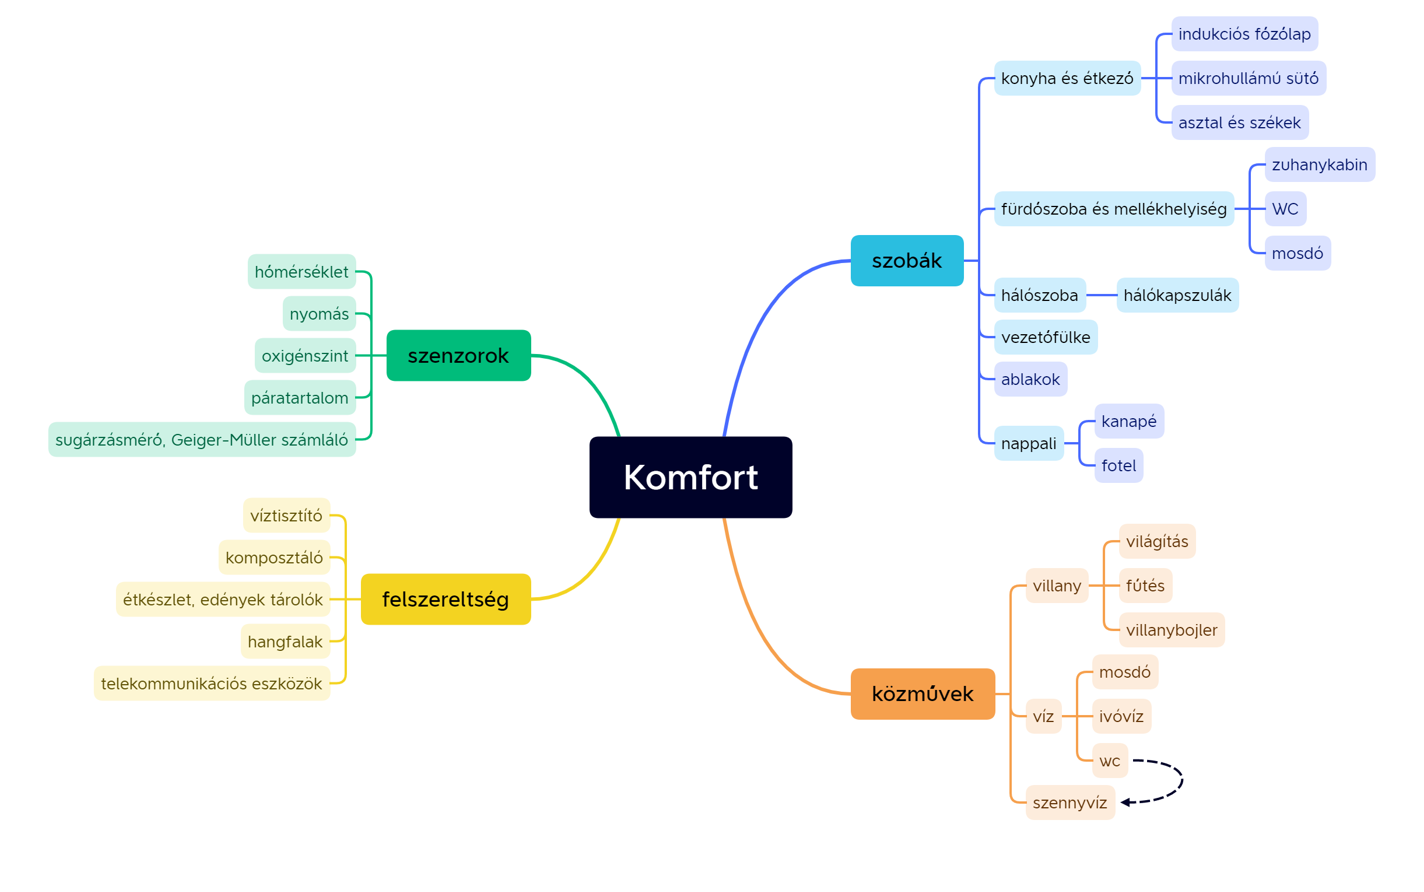
\includegraphics[scale=0.4]{images/komfort01.png}



\begin{itemize}
    \item Szobák száma: 5
    \item fertőtlenítés, sterilizálás
    \item vizsgálatvégző műszerek tárolása
    \item 
\end{itemize}

A marsjáróban állandó oxigénszint, hőmérséklet és páratartalom kell ehhez három szenzor van szükség.

Szenzorok:
\begin{itemize}
    \item hőmérséklet: $22^\circ C $ 
    \item páratartalom: 40-60 \%
    \item oxigénszint
    \item nyomás
    \item sugárzásmérő
\end{itemize}

\subsection{konyha és éléskamra}

25nm-es konyha és étkező
Egy ember napi 3 liter vízfogyasztással számolva 4 ember x 3liter x 20 nap = 240 l (minimum) tárolására alkalmas.
\begin{itemize}
    \item hűtőszekrény: mivel a Marson az átlaghőmérséklet $ -63^\circ C $ ezért a hűtésre fordított energiát a Mars légköréből biztosítják, hogy kevesebb kompressziós energiával lehessen a hűtést megoldani.
    \item indukciós főzőlap
    \item mosogatógép
    \item egyéb konyhai eszközök (mikrohullámú sütő, robotgép, edények) tárolására alkalmas szekrény
    \item evőeszközök: 4 pár étkészlet 4 darab pohár és bögre
    \item szelektív hulladék gyűjtésére kialakított tárolók
    \item 
\end{itemize}

\subsection{fürdőszoba}
\subsection{vezetőfülke}
\subsection{hálószoba}
\begin{itemize}
    \item hálókapszulák száma: 2 db (2m*0.5m*0.4m)
    \item Szobák: hálószoba 
    \item fertőtlenítés, sterilizálás
    \item vizsgálatvégző műszerek tárolása
    \item 
\end{itemize}
\subsection{nappali}



\section{References (??)}
\end{document}
